\documentclass{include/protokollclass}
% Main File - Based on protokollclass.cls
% Comments are mostly in English (and some in German, concerning the Praktikum)
% ------------------------------------------------------------------------------
% Further files in folder:
%  - include/cmds.tex (for macros and additional commands)
%  - include/kitlogo.pdf (for titlepage)
%  - lit.bib (bibtex bibliography database)
%  - include/titlepage.tex (for layout of titelpage)
% ------------------------------------------------------------------------------
% Useful Supplied Packages:
% amsmath, amssymb, mathtools, bbm, upgreek, nicefrac,
% siunitx, varioref, booktabs, graphicx, tikz, multicol





%% ---------------------------------------------
%% |    Informationen über dieses Protokoll    |
%% ---------------------------------------------
\newcommand{\praktikum}{P1}                % P1 oder P2
\newcommand{\semester}{WS21/22}            % z.B. "WS14/15" oder "SS15"

\newcommand{\wochentag}{Do}                % Mo, Di, Mi oder Do
\newcommand{\gruppennr}{7}                % Zweistellige Gruppennummer

\newcommand{\nachnamea}{Linn}             % Nachname des ersten Praktikanten
\newcommand{\vornamea}{Myriel}               % Vorname des ersten Praktikanten
\newcommand{\nachnameb}{Schwartz}           % Nachname des zweiten Praktikanten
\newcommand{\vornameb}{Arne}              % Vorname des zweiten Praktikanten

\newcommand{\emailadressen}{uhreq@student.kit.edu, ukjfu@student.kit.edu}
% optionale Angabe von Emailadresse(n) für den Kontakt mit dem Betreuer

\newcommand{\versuch}{Pendel} % Name des Versuchs
\newcommand{\versuchsnr}{80}               % bitte die korrekte Nummer dem 
                                           % Arbeitsplatz am Versuchstag 
                                           % entnehmen
\newcommand{\fehlerrechnung}{Nein}         % Ob Fehlerrechnung im Versuch 
                                           % durchgeführt wurde oder nicht

\newcommand{\betreuer}{Philip Schmid}      % Name des zuständigen Betreuers
\newcommand{\durchgefuehrt}{11.11.21}      % Datum, an dem der Versuch 
                                           % durchgeführt wurde




%% --------------------------------------
%% |    Settings for Word Separation    |
%% --------------------------------------
% Help for separation:
% In German package the following hints are additionally available:
% "- = Additional separation
% "| = Suppress ligation and possible separation (e.g. Schaf"|fell)
% "~ = Hyphenation without separation (e.g. bergauf und "~ab)
% "= = Hyphenation with separation before and after
% "" = Separation without a hyphenation (e.g. und/""oder)

% Describe separation hints here:
\hyphenation
{
    über-nom-me-nen an-ge-ge-be-nen
    %Pro-to-koll-in-stan-zen
    %Ma-na-ge-ment  Netz-werk-ele-men-ten
    %Netz-werk Netz-werk-re-ser-vie-rung
    %Netz-werk-adap-ter Fein-ju-stier-ung
    %Da-ten-strom-spe-zi-fi-ka-tion Pa-ket-rumpf
    %Kon-troll-in-stanz
}





% um die Titelseite per PDF-reader auszufüllen. Vorgefertigte Daten
% können in Datei 'data.tex' modifiziert werden.
%\setboolean{forminput}{true}
% um die Anmerkungen zu den Textfeldern anzeigen zu lassen
%\setboolean{showannotations}{true}
% Erneuern der Seitenzahl in jedem Kapitel
%\setboolean{chapResetPageNumb}{true}
% Einbinden der Kapitelnummer in der Seitenzahl
%\setboolean{chapWiseNumb}{true}
% english or ngerman (new german für neue deutsche Rechtschreibung statt german)
\SelectLanguage{ngerman}





%% -----------------------
%% |    Main Document    |
%% -----------------------
\begin{document}
    % Titlepage und ToC
    \FrontMatter

    % coordinates for background border
\newcommand{\diameter}{20}
\newcommand{\xone}{-15}
\newcommand{\xtwo}{160}
\newcommand{\yone}{15}
\newcommand{\ytwo}{-253}

\newcommand{\hoehea}{55}
\newcommand{\hoeheb}{55}




\begin{titlepage}
    % background border
    \begin{tikzpicture}[overlay]
    \draw[color=gray]  
            (\xone mm, \yone mm)
      -- (\xtwo mm, \yone mm)
    arc (90:0:\diameter pt) 
      -- (\xtwo mm + \diameter pt , \ytwo mm) 
        -- (\xone mm + \diameter pt , \ytwo mm)
    arc (270:180:\diameter pt)
        -- (\xone mm, \yone mm);
    \end{tikzpicture}
    
    % KIT logo
    \begin{textblock}{10}[0,0](4.5,2.5)
        
\includegraphics[width=.25\textwidth]{include/kitlogo.pdf}
    \end{textblock}
    \changefont{phv}{m}{n}    % helvetica
    \begin{textblock}{10}[0,0](5.5,2.2)
        \begin{flushright}
            \Large FAKULTÄT FÜR PHYSIK\\Praktikum Klassische Physik
        \end{flushright}
    \end{textblock}
    
    \begin{textblock}{10}[0,0](4.2,3.1)
        \begin{tikzpicture}[overlay]
        \draw[color=gray]
            (\xone mm + 5 mm, -8 mm)
         -- (\xtwo mm + \diameter pt - 5 mm, -8 mm);
        \end{tikzpicture}
    \end{textblock}
    
    \Large
    % Zeile 1
    \begin{textblock}{12}[0,0](3.58,4)
        \mytextfield{Prak.}{\praktikum}{0.9cm}{17pt}
                    {P1/P2}{2}{Praktikum}
    \end{textblock}
    \begin{textblock}{12}[0,0](5.53,4)
        \mytextfield{Semester}{\semester}{2.6cm}{17pt}
        {z.B. \glqq WS14/15\grqq\ oder \glqq SS15\grqq}{0}{Semester}
    \end{textblock}
    \begin{textblock}{12}[0,0](9.53,4)
        \mytextfield{Wochentag}{\wochentag}{1.3cm}{17pt}
                    {Mo/Di/Mi/Do}{2}{Wochentag}
    \end{textblock}
    \begin{textblock}{12}[0,0](12.88,4)
       \mytextfield{Gruppennr.}{\gruppennr}{1.06cm}{17pt}
                   {\#\#}{2}{Gruppennummer}
    \end{textblock}
    
    % Zeile 2
    \begin{textblock}{12}[0,0](3.58,4.55)
        \mytextfield{Name}{\nachnamea}{6cm}{17pt}
                    {}{0}{Name1}
    \end{textblock}
    \begin{textblock}{12}[0,0](9.53,4.55)
        \mytextfield{Vorname}{\vornamea}{6cm}{17pt}
                    {}{0}{Vorname1}
    \end{textblock}
    
    % Zeile 3
    \begin{textblock}{12}[0,0](3.58,5.1)
        \mytextfield{Name}{\nachnameb}{6cm}{17pt}
                    {}{0}{Name2}
    \end{textblock}
    \begin{textblock}{12}[0,0](9.53,5.1)
        \mytextfield{Vorname}{\vornameb}{6cm}{17pt}
                    {}{0}{Vorname2}
    \end{textblock}
    
    % Zeile 4
    \begin{textblock}{12}[0,0](3.64,5.65)
       \normalsize\mytextfield{Emailadresse(n)}{\emailadressen}{13.1cm}{10pt}
                              {Optional}{0}{Emailadressen}
    \end{textblock}
    
    % Zeile 5
    \begin{textblock}{12}[0,0](3.58,6.2)
        \mytextfield{Versuch}{\versuch\ (\praktikum-\versuchsnr)}{9.45cm}{14pt}
                    {z.B. \glqq Galvanometer (P1-13)\grqq\ oder \glqq %
                     Mikrowellenoptik (P2-15)\grqq}{0}{Versuch}
    \end{textblock}
    \begin{textblock}{12}[0,0](12.58,6.2)
       \mytextfield{Fehlerrech.}{\fehlerrechnung}{1.46cm}{17pt}
                   {Ja/Nein}{4}{Fehlerrechnung}
    \end{textblock}
    
    % Zeile 6
    \begin{textblock}{12}[0,0](3.58,6.75)
        \mytextfield{Betreuer}{\betreuer}{7cm}{17pt}{}{0}{Betreuer}
    \end{textblock}
    \begin{textblock}{12}[0,0](10.82,6.75)
        \mytextfield{Durchgeführt am}{\durchgefuehrt}{2.53cm}{17pt}
                    {TT.MM.JJ}{8}{Durchfuehrung}
    \end{textblock}
    
    % Querstrich
    \begin{textblock}{20}[0,0](0,7.1)\tiny\centering
        Wird vom Betreuer ausgefüllt.
    \end{textblock}
    \begin{tikzpicture}[overlay]
    \draw[color=gray]
        (\xone mm + 5 mm, -78 mm)
     -- (\xtwo mm + \diameter pt - 5 mm, -78 mm);
    \end{tikzpicture}
    
    % Zeile 1
    \begin{textblock}{12}[0,0](3.58,8)
        \myTtextfield{1. Abgabe am}{}{2.5cm}{17pt}
                     {}
    \end{textblock}
    \begin{textblock}{20}[0,0](8.3,8)
        \myTtextfield{Rückgabe am}{}{2.5cm}{17pt}
                     {}
    \end{textblock}
    
    % Block 1
    \begin{tikzpicture}[overlay]
    \draw[color=gray]  
        (\xone mm + 10 mm, -85.5 mm)
     -- (\xtwo mm + \diameter pt - 10 mm, -85.5 mm)
     -- (\xtwo mm + \diameter pt - 10 mm, -85.5 mm - \hoehea mm)
     -- (\xone mm + 10 mm, -85.5 mm - \hoehea mm)
     -- (\xone mm + 10 mm, -85.5 mm);
    \end{tikzpicture}
    
    \begin{textblock}{20}[0,0](4,8.57)
        Begründung:
    \end{textblock}
    
    % Zeile 2
    \begin{textblock}{12}[0,0](3.58,11.85)
        \myTtextfield{2. Abgabe am}{}{2.5cm}{17pt}
                     {}
    \end{textblock}
    
    % Block 2
    \begin{tikzpicture}[overlay]
    \draw[color=gray]  
        (\xone mm + 10 mm, -167 mm)
     -- (\xtwo mm + \diameter pt - 10 mm, -167 mm)
     -- (\xtwo mm + \diameter pt - 10 mm, -167 mm - \hoehea mm)
     -- (\xone mm + 10 mm, -167 mm - \hoehea mm)
     -- (\xone mm + 10 mm, -167 mm);
    \end{tikzpicture}
    \begin{textblock}{12}[0,0](4.25,12.24)
        {Ergebnis:~~~~+~~~/~~~0~~~/~~~-}
    \end{textblock}
    \begin{textblock}{12}[0,0](9.1,12.24)
        {Fehlerrechnung:~~~Ja~~~/~~~Nein}
    \end{textblock}
    \begin{textblock}{12}[0,0](4.05,12.9)
        \myTtextfield{Datum}{}{2.5cm}{17pt}
                     {}
    \end{textblock}
    \begin{textblock}{12}[0,0](8.9,12.9)
        \myTtextfield{Handzeichen}{}{5.5cm}{17pt}
                     {}
    \end{textblock}
    \begin{textblock}{12}[0,0](4,13.4)\Large
        {Bemerkungen:}
    \end{textblock}
    
    
    
    % lowest text blocks concerning the KIT
    \begin{textblock}{10}[0,0](4,16.8)
        \tiny{KIT -- Universität des Landes Baden-Württemberg und nationales %
              Forschungszentrum in der Helmholtz-Gemeinschaft}
    \end{textblock}
    \begin{textblock}{10}[0,0](14,16.75)
        \large{\textbf{www.kit.edu}}
    \end{textblock}
\end{titlepage}
 %\cleardoublepage

    \begingroup \let\clearpage\relax    % in order to avoid listoffigures and
    \tableofcontents                    % listoftables on new pages
    \listoffigures
    \listoftables
    \endgroup
    %\cleardoublepage



    % Contents
    \MainMatter
    
    %\emptychapter[1]{Messprotokoll 1}{} % usage: \emptychapter[page displayed 
                                        %        in toc]{name of the chapter}
    %\pseudochapter[3]{Messprotokoll 2}  % usage: \pseudochapter[number of pages 
                                        %        added]{name of the chapter}
    
    \chapter{Reversionspendel}
    \section{Reduzierte Pendellänge}

Es soll vorbereitend die reduzierte Pendellänge berechnet werden, also die Länge, die ein mathematisches Pendel haben würde (eine punktförmige Masse mit einem Faden mit vernachlässigbarer Masse), damit es mit gleicher Schwingungsdauer schwingen würde, wie das zu beschreibende physikalische Pendel. Das physikalische bzw. Reversionspendel Abb \ref{fig:Versuch 1.2}, für das die reduzierte Pendellänge berechnet werden soll, besteht aus einem zylindrischen, an einem Ende drehbar aufgehängte Stab der Länge l.

\begin{figure}[ht]
    \centering
    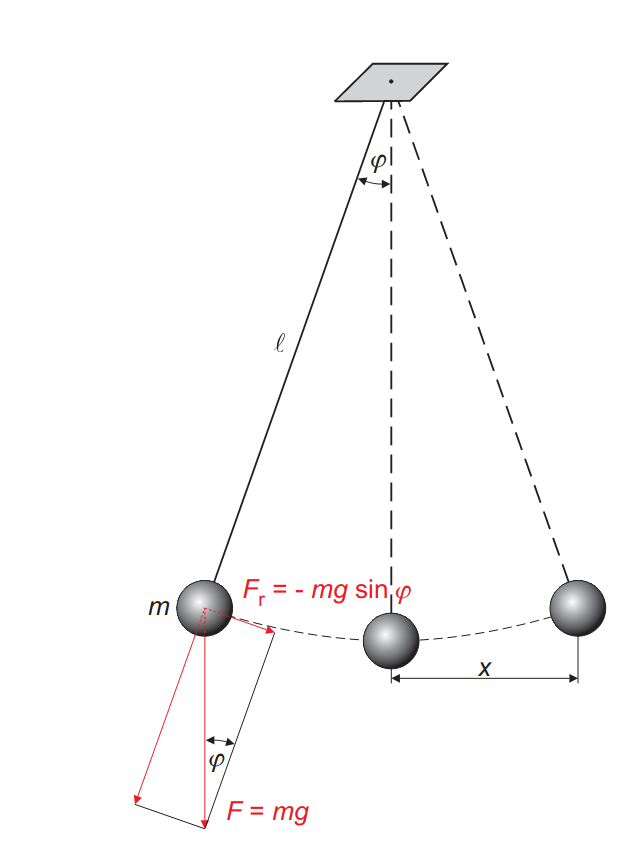
\includegraphics[scale=0.3]{Pendel/Protokoll/fig/Mathematisches Pendel.png}
    \caption{Mathematisches Pendel}
    \label{fig:Mathematisches Pendel}
    Quelle: Eichler Kronfeld Sahm "Das Neue Physikalische Grundpraktikum"
\end{figure}

\begin{figure}[ht]
    \centering
    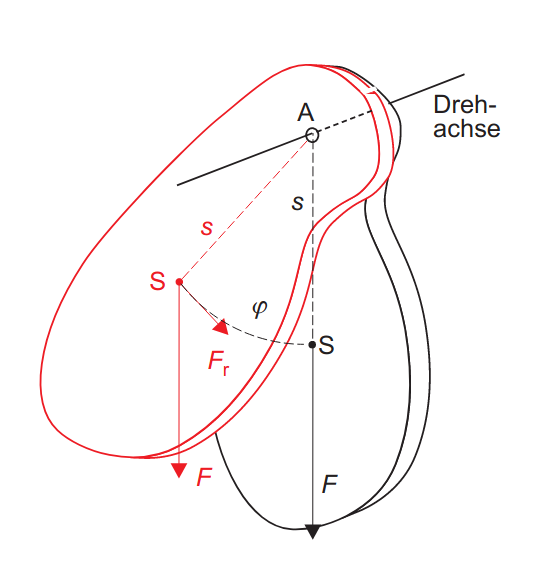
\includegraphics[scale=0.3]{Pendel/Protokoll/fig/Physikalisches Pendel.png}
    \caption{Physikalisches Pendel}
    \label{fig:Physikalisches Pendel}
    Quelle: Eichler Kronfeld Sahm "Das Neue Physikalische Grundpraktikum"
\end{figure}

\begin{figure}[ht]
    \centering
    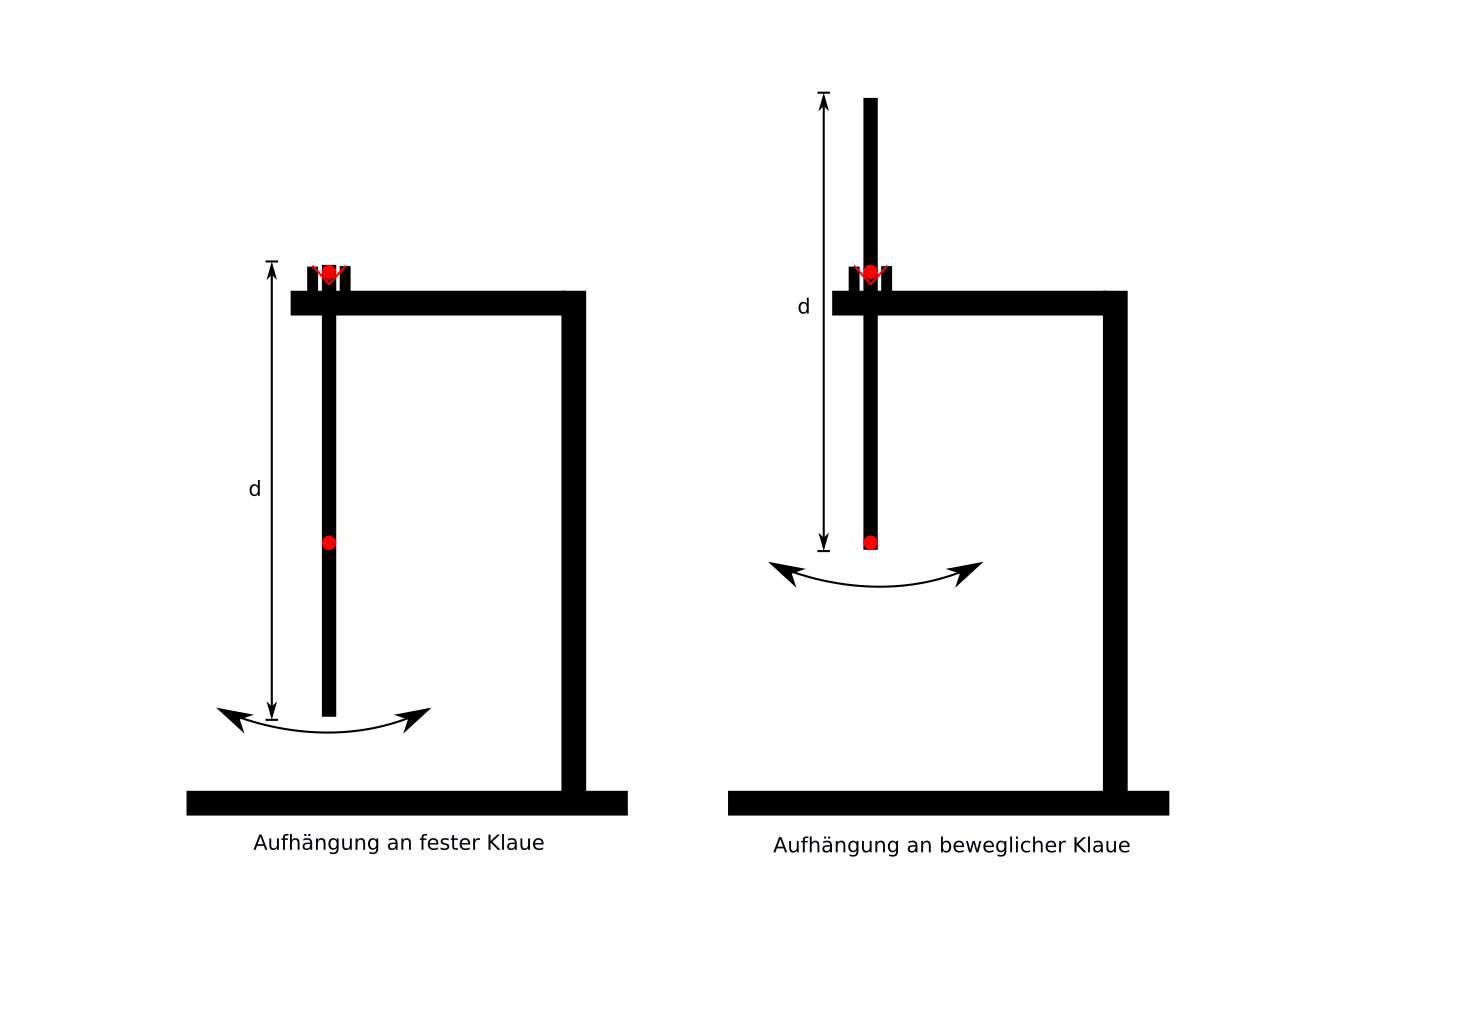
\includegraphics[scale=0.8]{Pendel/Protokoll/fig/Versuch 1.2.png}
    \caption{Physikalisches Pendel zur bestimmung der Fallbeschleunigung}
    \label{fig:Versuch 1.2}
\end{figure}

Nach der Grundgleichung für Drehbewegungen gilt:

\begin{equation} \label{Grundgleichung Drehbewegung}
    M = I \cdot \ddot{\varphi}
\end{equation}

wobei $M$ das rücktreibende Drehmoment, $I$ das Trägheitsmoment des Pendels und $\ddot{\varphi}$ die Winkelbeschleunigung ist. Für das rücktreibende Drehmoment gilt: $M = -m \cdot g \cdot s \cdot \sin{\varphi}$, wobei $m$, die Masse des Pendels, $g$ die Erdbeschleunigung und $s$ die Pendellänge ist. Mit der Kleinwinkelnäherung $\sin{\varphi}$ folgt nach Einsetzen in Gleichung \ref{Grundgleichung Drehbewegung}:

\begin{equation} \label{Schwingungsgleichung eines physikalischen Pendels}
\ddot{\varphi} + \omega^2\varphi = 0
\Rightarrow \varphi = e^{i \omega t} \text{, mit } \omega = \sqrt{\frac{mgs}{I}}
\end{equation}

Mit dem Ergebnis für die Kreisfrequenz $\omega$ lässt sich nun die Persiodendauer $T$ berechnen:

\begin{equation}
    T = \frac{2\pi}{\omega} = 2 \pi \sqrt{\frac{I}{mgs}}
\end{equation}

Das Trägheitsmoment eines Zylinders mit einer homogenen Masseverteilung ist gegeben durch $I_Z = \frac{1}{3} ml^2$. Der Abstand zwischen Schwerpunkt und Drehpunkt des Zylinders ist$s = l/2$. Daraus folgt für die Periodendauer des physikalischen Pendels:

\begin{equation}
    T = 2 \pi \sqrt{\frac{I}{mgs}} = 2 \pi \sqrt{\frac{\frac{1}{3} l^2}{mg\frac{l}{2}}} = 2 \pi \sqrt{\frac{2l}{3g}}
\end{equation}

Durch einen Vergleich mit der Periodendauer eines mathematische Pendels:

\begin{equation} \label{Periodendauer mathematisches Pendel}
   T_m = 2 \pi \sqrt{\frac{l_r}{g}} 
\end{equation} 

lässt sich erkennen, dass die reduzierte Pendellänge $l_r = \frac{2}{3}l$ beträgt.

Weiter soll vorbereitend gezeigt werden, dass eine zusätzlich angebrauchte Masse bei $l_r$  keine Veränderung der Periodendauer hervorruft. Also gilt für $I^\prime = m^\prime (\frac{2}{3}l)^2$ und für $s^\prime = \frac{2}{3}l$

\begin{equation}
    T^\prime = 2 \pi \sqrt{\frac{I + I^\prime}{mgs+m^\prime g s^\prime }} = 2\pi \sqrt{ \frac{ (\frac{m}{2} + \frac{2}{3} m^\prime) \frac{2}{3}l^2} { (\frac{m}{2} + \frac{2}{3}m^\prime)g l  }} \equiv T
\end{equation}

Mit dieser Erkenntnis lässt sich argumentieren, dass die Klauen, an denen das Pendel aufgehängt wird, keine Änderung der Periodendauer mit sich bringen.

\section{Bestimmung der Fallbeschleunigung g mit Hilfe des Reversionspendels}

Aus Gleichung \ref{Periodendauer mathematisches Pendel} erhält man durch umformen eine Formel für die Fallbeschleunigung: 

\begin{equation} \label{Fallbeschleunigung mathematisches Pendel}
    g = l_r \frac{4 \pi^2}{T^2}
\end{equation}

wobei in diesem Versuchsteil $l_r$ experimentell bestimmt werden soll, um somit die Fallbeschleunigung experimentell zu bestimmen. Dabei ist die Periodendauer gleich um beiden Schneiden, wenn $d = l_r$ gilt, wobei $d$ der Abstand der beiden Schneiden ist. Für die Bestimmung von $l_r$ wird eine Messreihe für verschiedene Abstände $d$ der beiden Schneiden angefertigt (Abb. \ref{fig:Pendel Versuch 1.1}). Wie man an dem Plot erkennen kann, folgt die Periodendauer für die Aufhängung an der festen Schneide einer Geraden, während dies für die bewegliche Schneide nicht der Fall ist, deshalb werden für die lineare Regression (Abb \ref{fig:Pendel Versuch 1.1 Fit}) nur Datenpunkte in der Nähe vom Schnittpunkt gewählt, wo der Verlauf näherungsweise linear ist. Die reduzierte Länge erhält man nun, indem man den Schnittpunkt der beiden angepassten Gerade berechnet:

\begin{align} 
    \nonumber y_{fest} &=  1.4383s + 0.252 \cdot \frac{s}{m} x\\
    \nonumber y_{beweglich} &= 2.2040s -0.953 \cdot \frac{s}{m} x
\end{align}

Gleichsetzen und auflösen nach x liefert nun:

    $$x=l_r \approx 0.6354m $$
    Einsetzen liefert nun für die Periodendauer:
    $$T = y_{fest}(l_r) = y_{beweglich}(l_r) = 1.598 s$$

Damit erhalten wir nach einsetzen in die Gleichung \ref{Fallbeschleunigung mathematisches Pendel}:

$$ g = l_r \frac{4 \pi}{T^2} \approx 9.823 $$

Der Literaturwert für die Fallbeschleunigung beträgt $g=9.81 \frac{m}{s^2}$, unsere Abweichung beträgt demnach nur ungefähr $0.1 \% $\\
Mögliche Fehlerquellen für die Abweichung sind:
\begin{itemize}
    \item Luftreibung
    \item Reibung der Aufhängung
    \item Ein zu groß gewählter Auslenkwinkel (Kleinwinkelnäherung gilt nicht mehr)
    \item Nicht gut geeichte Lichtschranke
    \item Beim Loslassen des Pendels eine Anfangsgeschwindigkeit übertragen, die das Ergebnis verfälscht
    \item Zufällige Streuung der Messwerte aufgrund der Ungenauigkeit der Lichtschranke ($\Rightarrow$ mehr Messwerte)
\end{itemize}

\begin{figure}[ht]
    \centering
    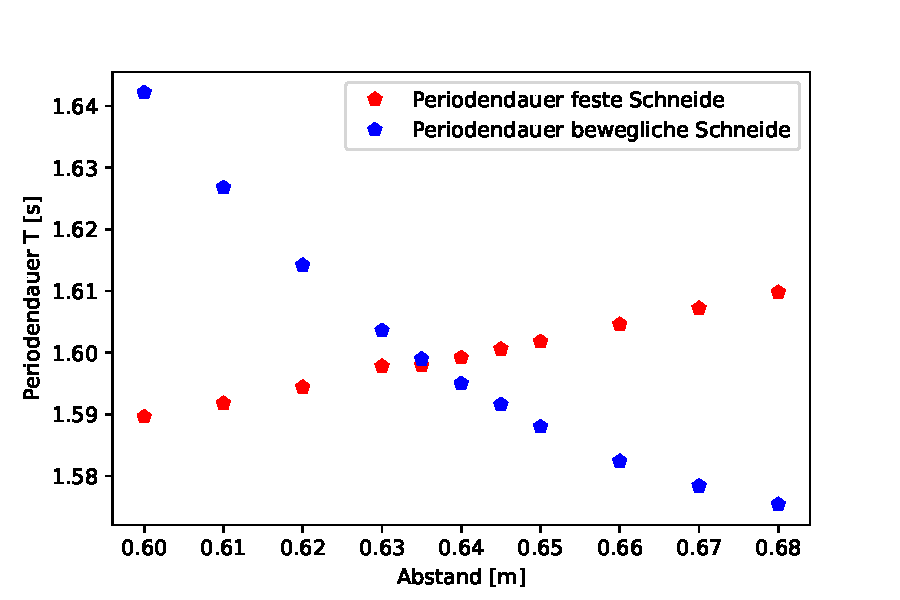
\includegraphics[scale=0.8]{Pendel/Protokoll/fig/Pendel Versuch 1.2.pdf}
    \caption{Daten Versuch 1.2}
    \label{fig:Pendel Versuch 1.1}
\end{figure}

\begin{figure}[ht]
    \centering
    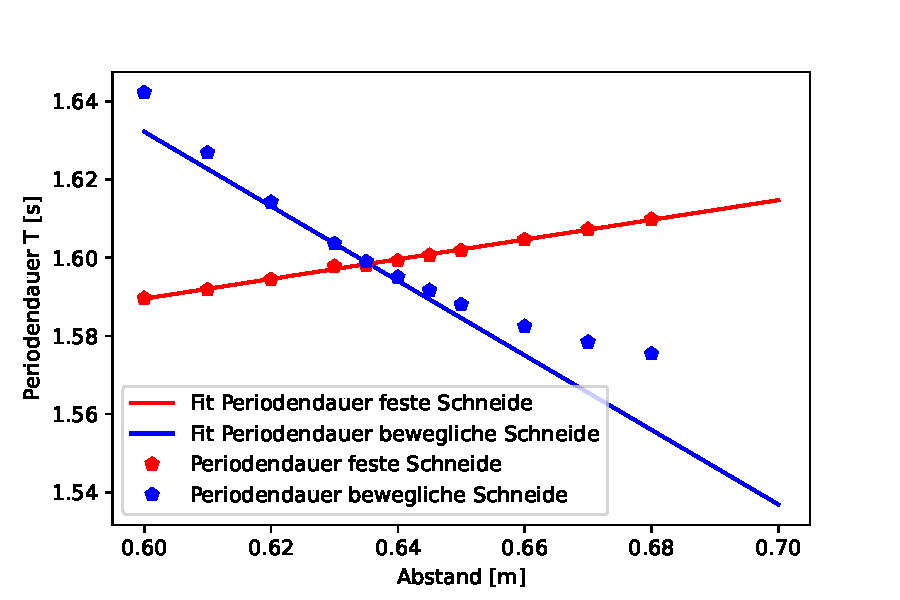
\includegraphics[scale=0.8]{Pendel/Protokoll/fig/Pendel Versuch 1.2 Fit.pdf}
    \caption{Fit Versuch 1.2}
    \label{fig:Pendel Versuch 1.1 Fit}
\end{figure}
    \chapter{Fadenpendel}
    \section{Aufbau}

Der Aufbau besteht aus einem dünnen, von der Decke hängenden Stahlseil, an dessen Ende eine Metallkugel befestigt ist. An der Wand hinter dem Pendel befindet sich eine Winkelskala. Die Messungen werden erneut mit Hilfe einer Lichtschranke duchgeführt.

\section{Bestimmung der Fallbeschleunigung}

\section{Mathematische Grundlagen}

Um die Fallbeschleunigung g der Erde mit Hilfe eines Pendels zu bestimmen, muss man zunächst eine Entscheidung darüber fällen, ob man mit dem Modell eines mathematischen oder eines physikalischen Pendels modellieren sollte.
In diesem Versuch wird das physikalische Pendel verwendet, da die Versuchbedinungen nicht idealisiert waren und das mathematische Modell daher zu ungenau wäre.

Da das Pendel für diesen Versuch um kleinen Winkel von ca. 5° augelenkt wurde, wird auf die Kleinwinkelannäherung des physikalischen Pendels zurückgegriffen

\begin{align}
	\label{eq:physikalisches-pendel}
	T = 2 \pi \sqrt{\frac{\theta}{m g d}}  \implies T^2 = 4 \pi^2 \frac{\theta}{m g d} \implies g = \frac{4 \pi^2 \theta}{m d T^2} .
\end{align}

Das Trägheitsmoment $\theta$ des Pendels setzt sich aus dem Trägheitsmoment der Kugel und dem Trägheitsmoment nach dem Satz von Steiner zusammen.
Da man die Kugel als Kugelkreisel ansehen kann, ergibt sich vereinfacht

\begin{align}
	\theta = \theta_\text{Kugel} + \theta_\text{Steiner} = \frac{2}{5} m r^2 + m d^2 .
\end{align}

Nach einsetzen in \ref{eq:physikalisches-pendel} ergibt sich

\begin{align}
	\label{eq:ortsfaktor}
	g = \frac{4 \pi^2 m (\frac{2}{5} r^2 + d^2)}{m d T^2} = 4 \pi^2 \frac{\frac{2}{5} r^2 + d^2}{d T^2}
\end{align} .

Die Periodendauer $T$ errechnet sich aus den Messwerten des Versuchs, die Länge $d$ des Pendelfadens ist als 2,355m gegeben und mit einem systematischen Fehler von 3mm behaftet.

Zuletzt wird der Radius der Kugel benötigt. Um diesen zu ermitteln, wurde der Durchmesser $D$ der Kugel dreimal mit einem Messschieber gemessen und über die Werte gemittelt.

\section{Durchführung und Auswertung}

Während dem Versuch wurde das Pendel 10 mal um einen kleinen Winkel von ca. 5° augelenkt und jeweils die Zeit gemessen, bis die vorgegebene Zahl an Perioden durchlaufen wurde.

\begin{table}[h!]
    \begin{center}
        \caption{Messwerte von Versuch 2.1}
        \begin{tabular}{cccc}
            \hline
            Perioden  & $T in s$  \\
            \hline
            1                   & 3,051		\\
            3                   & 9,206		\\
            5                   & 15,360	\\
            7                   & 21,515	\\
            9                   & 27,672	\\
            11                  & 33,828	\\
            13                  & 39,985	\\
            15                  & 46,145	\\
	        17                  & 52,300	\\
	        19                  & 58,471	\\
            \hline
            \label{tab:2_1-werte}
        \end{tabular}
    \end{center}
\end{table}


Die Berechnung der Periodendauer wird durch Regression ausgeführt.

Aus der Regression ergibt sich für $T$ ein Wert von $3.079s$, mit einer statistischen Fehlerbehaftung von $0,000018s$.

Der Radius der Kugel errechnet sich wie folgt:

$D_M = \frac{D_1 + D_2 + D_3}{3}$
$r = \frac{D_M}{2}$

Der Durchmesser der Kugel wurde zu $0,060m$, $0,059m$ und $0,060m$ gemessen.
Aufgrund der Ungenauigkeit des Messchiebers, werden die $D_i$ mit einem systematischen Fehler von $0,005m$ behaftet, wozu noch eine Standardabweichung zu $0,0006$m als statistischer Fehler hinzukommt.

Es ergibt sich demnach $r = 0,03m$ mit einem statistischen Fehler von $0,0003m$ und einem einem systematischen Fehler von $0,0025m$.

Nach \ref{eq:ortsfaktor} ergibt sich

$g = 9,8075\frac{m}{s^2}$

Zur Fehlerrechnung wird Gaußsche Fehlerfortpflanzung verwendet. Dies ist möglich, da man aufgrund der ungenauen Messmethode den Zusammenhang von r und d vernachlässigen kann und somit alle Fehler unkorreliert sind.

\section{Abhängigkeit der Schwingungsdauer von der Schwingungsweite}

Im zweiten Teil des Versuches wird die Beziehung zwischen der Schwingungsdauer und dem Auslenkungswinkel des Pendels untersucht.
Dazu wurde die Periodendauer jeweils für Winkel von 5° bis 60° in fünfer Schritten gemessen,
wobei für jede Messung 5 Perioden durchlaufen wurden.
Das Einstellen der Auslenkung des Pendels war durch die Natur des Versuchsaufbaus nicht genau möglich.
Um zumindest grobe Fehler zu vermeiden, wurde das Pendel von einer Person unter der Anleitung einer zweiten, weiter entfernten Person, ausgelenkt.

\section{Mathematische Grundlagen}

Die gemessenen Daten sollen mit einer Vorhersage verglichen werden.
Diesmal wird die Vorhersage mit dem Modell des mathematischen Pendels modelliert:

\begin{align}
	\ddot{\phi}(t) + \frac{g}{l} \cdot \sin ( \phi (t)) = 0
\end{align}

Analytisch ist diese Differenzialgleichung nicht lösbar, mit Hilfe der Taylorentwicklung kann man sie jedoch genügend annähern:

\begin{align}
	T(\phi) & = T_0 \sum_{n=0}^{\infty} \left( \frac{\left(2n\right)!}{\left(2^{n}n!\right)^2} \right)^2 \sin^{2n} \left(\phi /2\right) \\
& = T_0\cdot\left(1+\left(\frac{1}{2}\right)^2 \cdot \sin^2\left(\frac{\phi}{2}\right)+\left(\frac{1\cdot 3}{2\cdot 4}\right)^2 \cdot \sin^4\left(\frac{\phi}{2}\right) + \dots\right)
\end{align}

$T_0$ ist die Periodendauer für kleine Winkel, die aus dem ersten Versuchsteil übernommen werden kann.

\section{Auswertung}

\begin{table}[h!]
    \begin{center}
        \caption{Messwerte von Versuch 2.2}
        \begin{tabular}{cccc}
            \hline
            Auslenkwinkel in $ ^{\circ}$ & T in s \\
            \hline
            5                  & 15,357 \\
            10                & 15,380 \\
            15                & 15,409 \\
            20                & 15,463 \\
            25                & 15,524 \\
            30                & 15,609 \\
            35                & 15,709 \\
            40                & 15,820 \\
            45                & 15,950 \\
            50                & 16,057 \\
            55                & 16,257 \\
            60                & 16,423 \\
            \hline
            \label{tab:2_2-werte}
        \end{tabular}
    \end{center}
\end{table}


Die Messung und die Vorhersage werden nun zum visuellen Vergleich gemeinsam geplottet.


    \chapter{Gekoppeltes Pendel}
    \section{Aufbau und Vorbereitung}

Im letzten Versuch wird das Verhalten gekoppelter Pendel untersucht. Der Aufbau besteht aus zwei mit einer Feder gekoppelten Stabpendeln, an denen jeweils eine Massescheibe angebracht ist.
Bevor man die Pendel koppelt, muss jedoch gesichert sein, dass die Pendel sich auch identisch verhalten.
Dazu werden zunächst der Dreh- und Massenpunkt festgelegt und dann die Periodendauern je Pendel gemessen und nach linearer Regression verglichen.

\begin{align}
    l &= \SI{80}{cm} \\
    L &= \SI{111}{cm} \\
    a &= \SI{31}{cm} \\
    m_{\text{Massescheibe}} &= \SI{1221}{g}
\end{align}

\begin{table}[h!]
    \begin{center}
        \caption{Zeiten für unterschiedliche Periodendauern beider Pendel}
        \begin{tabular}{ccc}
            \hline
            Anzahl Perioden & Zeit linkes Pendel in $\SI{}{s}$ & Zeit rechtes Pendel in $\SI{}{s}$ \\
            \hline
            3  & $\SI{5,51}{}$ & $\SI{5,36}{}$ \\
            5  & $\SI{9,09}{}$ & $\SI{8,84}{}$  \\
            7  & $\SI{12,53}{}$ & $\SI{12,51}{}$  \\
            9  & $\SI{15,98}{}$ & $\SI{16,08}{}$ \\
            \hline
            \label{tab:Schwingungen-Pendel-einzeln}
        \end{tabular}
    \end{center}
\end{table}

\begin{figure}[h!]
    \centering
    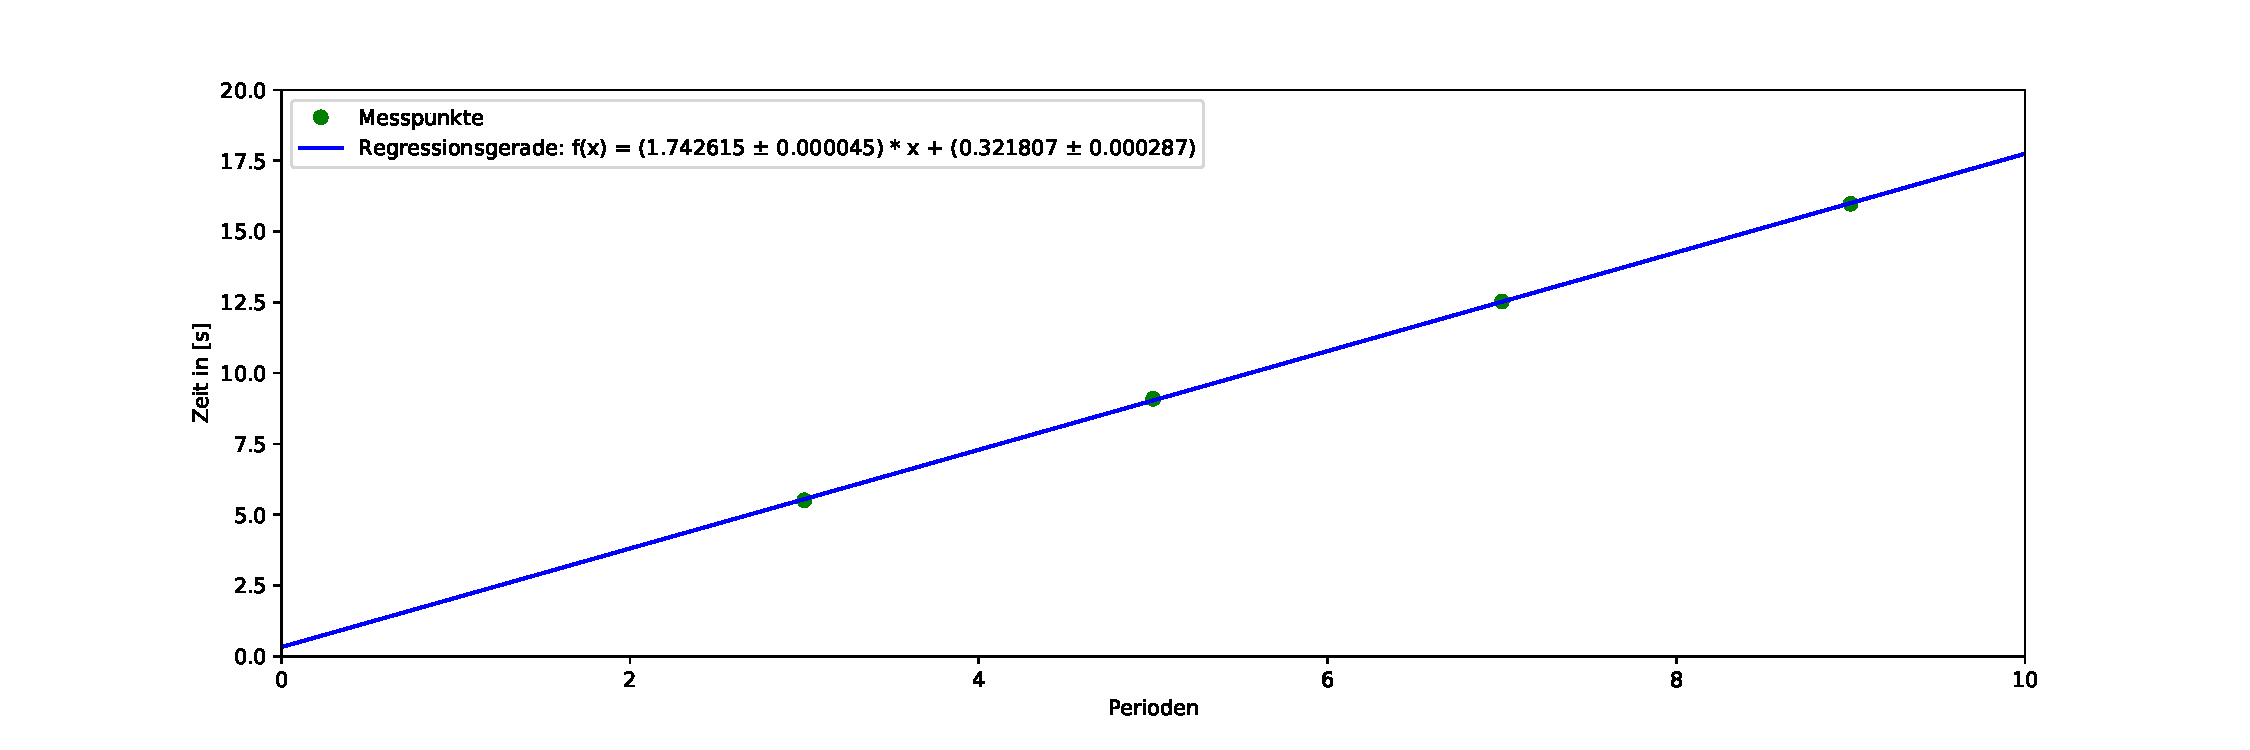
\includegraphics[scale=0.4]{./Pendel/Protokoll/fig/Koppelpendel_Regression_1.pdf}
    \caption{Plot der Messpunkte und der Regression für das linke Pendel}
    \label{fig:Reg_links}
\end{figure}

\begin{figure}[h!]
    \centering
    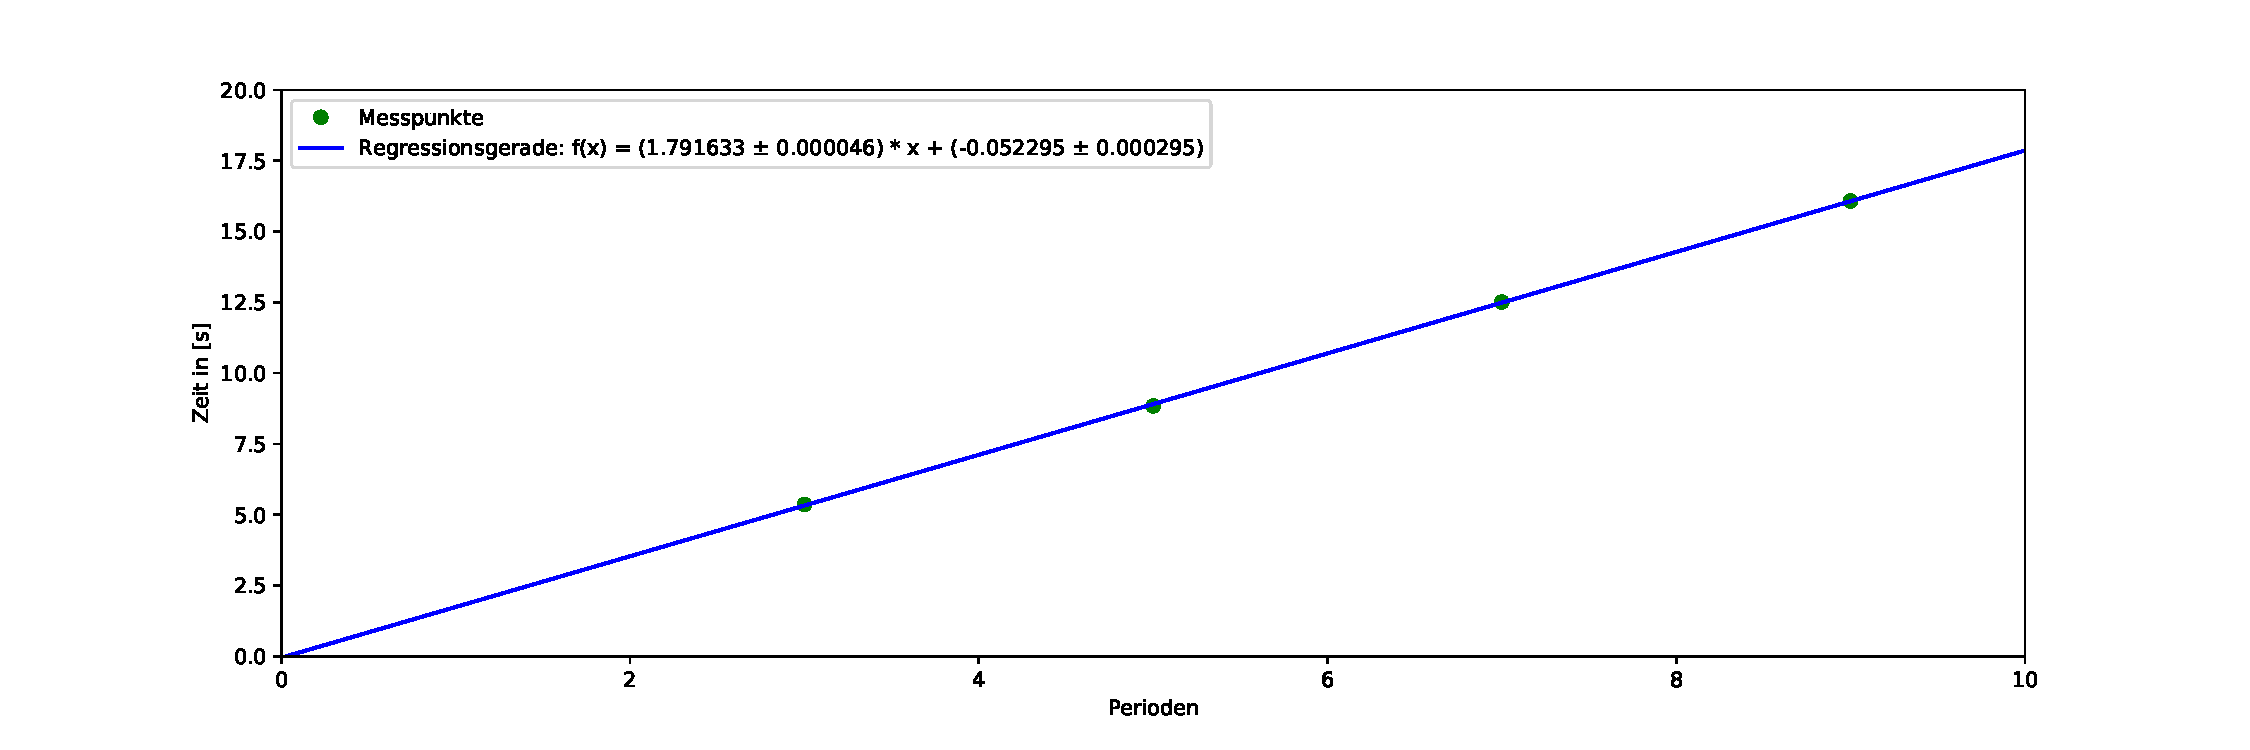
\includegraphics[scale=0.4]{./Pendel/Protokoll/fig/Koppelpendel_Regression_2.pdf}
    \caption{Plot der Messpunkte und der Regression für das rechte Pendel}
    \label{fig:Reg_rechts}
\end{figure}

\begin{table}[h!]
    \begin{center}
        \caption{Parameter lineare Regression}
        \begin{tabular}{ccc}
            \hline
            Pendel             & $m$ in $\SI{}{s}$ & $c$ in $\SI{}{s}$ \\
            \hline
            links              & $\SI{1,66(2)}{}$ & $\SI{0,8(130)}{}$ \\
            rechts             & $\SI{1,71(21)}{}$ & $\SI{0,45(135)}{}$  \\
            \hline
            Mittelwert         & $\SI{1.69(21)}{}$ & $\SI{0,063(132)}{}$ \\
            \hline
            \label{tab:Schwingungen-einzeln-Regression}
        \end{tabular}
    \end{center}
\end{table}


Da die Parameter des linken und des rechten Pendels nur gering von einander abweichen, kann man die beiden Pendel als identisch ansehen.


\clearpage

\section{Fundamentalschwingung}

Zur Analyse der Fundamentalschwingung werden die Pendel nun mit einer geeigneten Feder verbunden und die Periodendauer von Hand per Stoppuhr gemessen.
Geeignet bedeutet hier, dass die Federkonstante nicht zu groß sein sollte, da die Pendel sonst so schnell schwingen, dass die Zeit nicht mehr akkurat gestoppt werden kann.
Es wurde für zwei Koppellängen gemessen, wobei "Koppellänge" den Abstand ziwschen Drehpunkt und Federbefestigung bezeichnet.

\section{Auswertung}

\begin{table}[h!]
    \begin{center}
        \caption{Schwingungsdauern in $\SI{}{s}$}
        \begin{tabular}{cccc}
            \hline
            Koppellänge in $\SI{}{cm}$ & Periodenanzahl & gleichphasig   & gegenphasig    \\
            \hline
            \multirow{4}{*}{31}        & 3              & $\SI{5,37}{}$  & $\SI{4,70}{}$  \\
                                       & 5              & $\SI{8,79}{}$  & $\SI{7,90}{}$  \\
                                       & 7              & $\SI{12,29}{}$ & $\SI{10,83}{}$ \\
                                       & 9              & $\SI{15,9}{}$ & $\SI{14,03}{}$ \\
            \hline
            \multirow{4}{*}{28}        & 3              & $\SI{5,40}{}$  & $\SI{4,82}{}$  \\
                                       & 5              & $\SI{8,85}{}$  & $\SI{8,00}{}$  \\
                                       & 7              & $\SI{12,27}{}$ & $\SI{11,02}{}$ \\
                                       & 9              & $\SI{15,96}{}$ & $\SI{14,11}{}$ \\
            \hline
            \label{tab:Koppellaenge-Messwerte}
        \end{tabular}
    \end{center}
\end{table}

Die Auswertung geschieht erneut über Regression.

\begin{figure}[h!]{}
    \begin{center}
        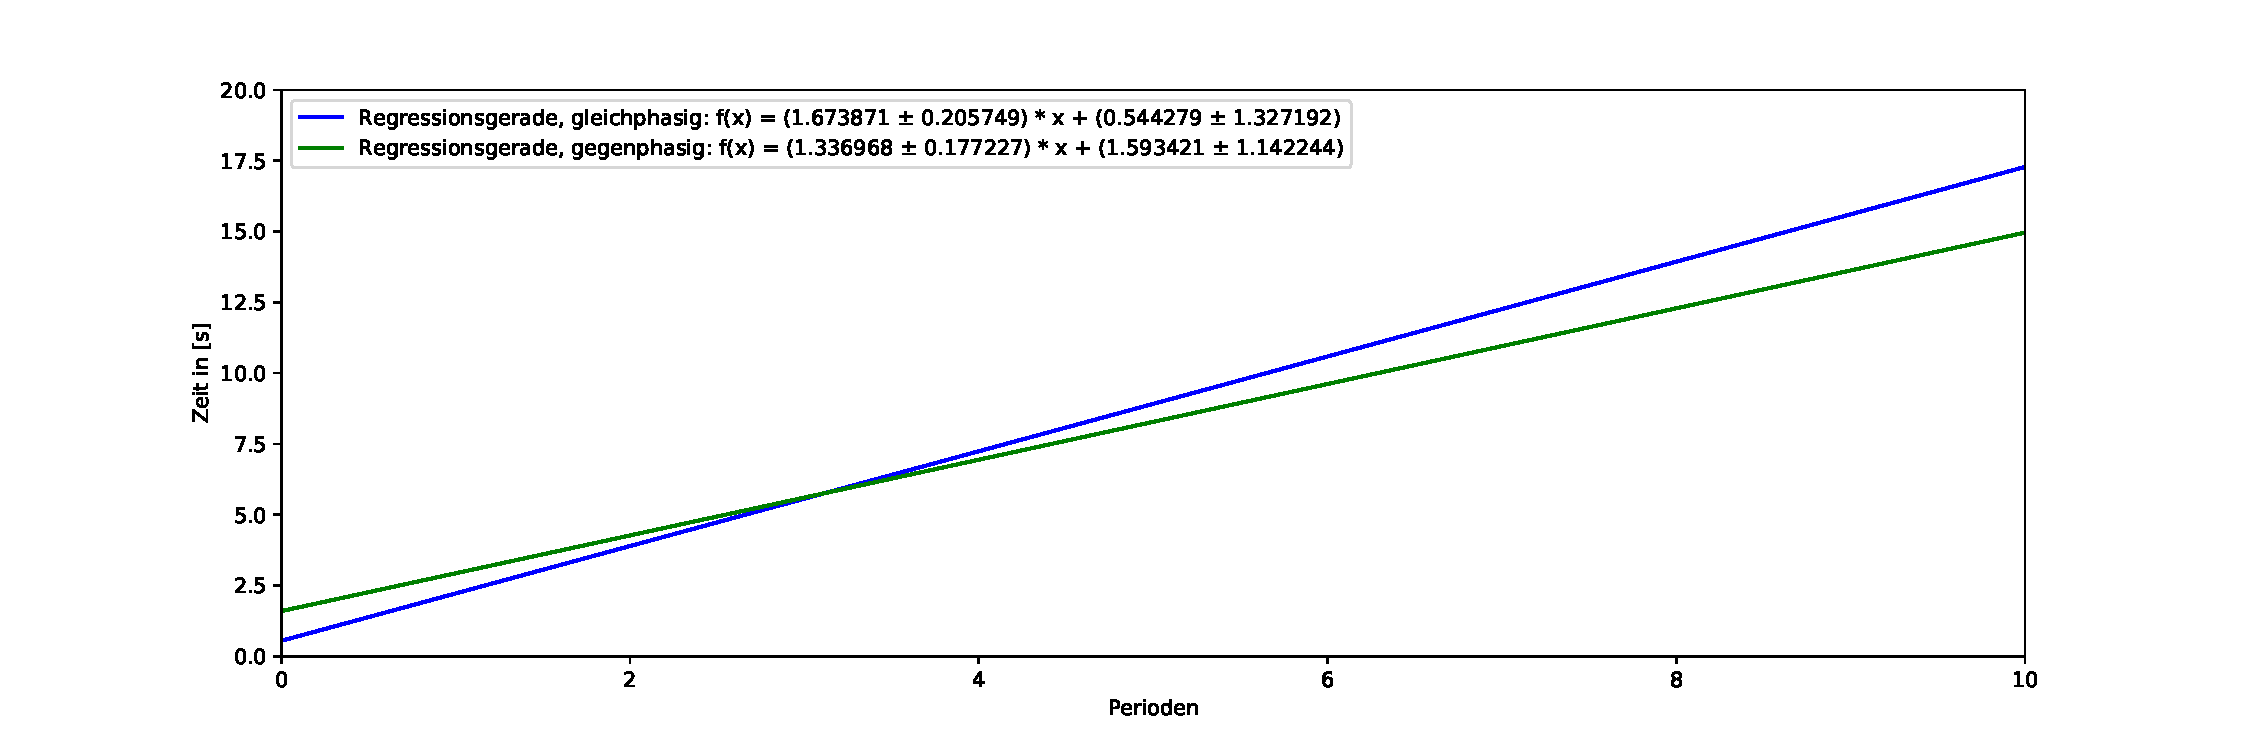
\includegraphics[scale = 0.4]{./Pendel/Protokoll/fig/Koppelpendel_Regression_3.pdf}
        \caption{Regression der Schwingungsdauern der gekoppelten Oszillatoren,  Kopplungslänge 31cm}
        \label{fig:Schwingungsdauern-gekoppelte-Oszillatoren1}
    \end{center}
\end{figure}

\begin{figure}[h!]{}
    \begin{center}
        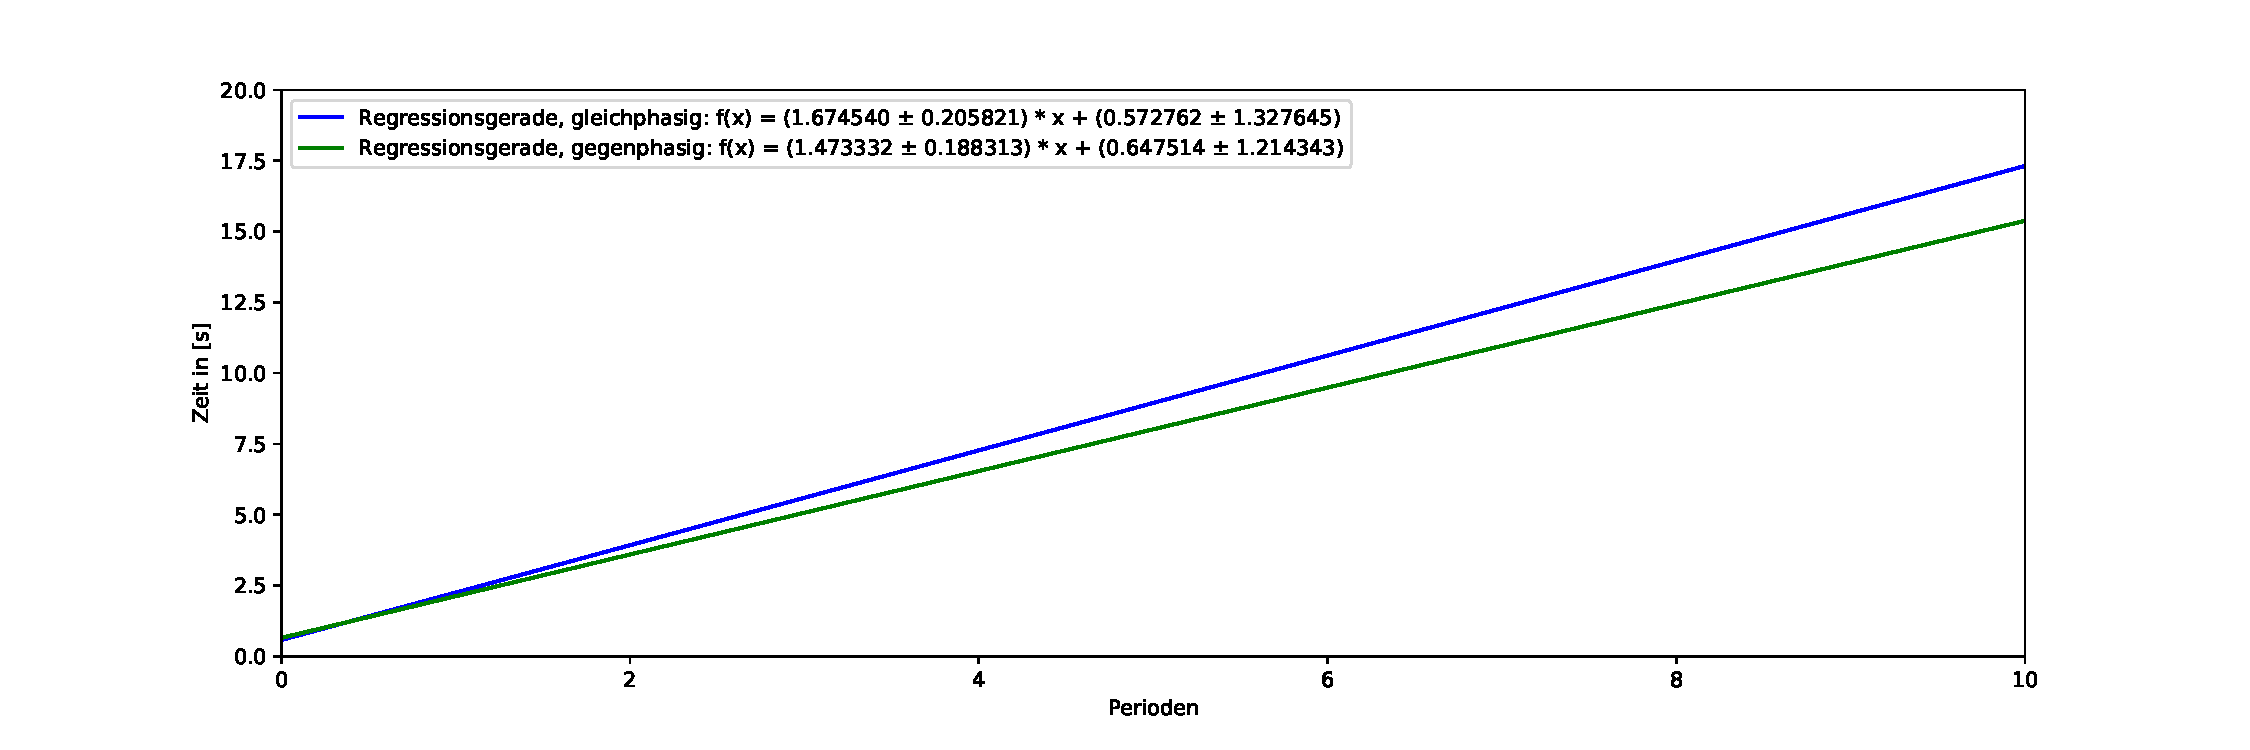
\includegraphics[scale=0.4]{./Pendel/Protokoll/fig/Koppelpendel_Regression_4.pdf}
        \caption{Regression der Schwingungsdauern der gekoppelten Oszillatoren, Kopplungslänge 28cm}
        \label{fig:Schwingungsdauern-gekoppelte-Oszillatoren2}
    \end{center}
\end{figure}


\begin{table}[h!]
    \begin{center}
        \caption{Schwingungsdauern in $\SI{}{s}$}
        \begin{tabular}{cccc}
            \hline
            Koppellänge in $\SI{}{cm}$ & Schwingungsform & m in $\SI{}{s}$   & c in $\SI{}{s}$ \\
            \hline
            \multirow{4}{*}{31}        & gleichphasig    & $\SI{1,67(21)}{}$ & $\SI{0,54(133)}{}$  \\
                                       & gegenphasig     & $\SI{1,34(18)}{}$ & $\SI{1,59(114)}{}$  \\
            \hline
            \multirow{4}{*}{28}        & gleichphasig    & $\SI{1,68(21)}{}$ & $\SI{0,57(133)}{}$  \\
                                       & gegenphasig     & $\SI{1,47(19)}{}$ & $\SI{0,65(121)}{}$  \\
            \hline
            \label{tab:Koppellaenge-Regressionswerte}
        \end{tabular}
    \end{center}
\end{table}

Vergleicht man die Messwerte für die gekoppelten Pendel mit denen der einzelnen Pendel, zeigt sich, dass bei gleichphasiger Schwingung kaum ein Unterschied vorhanden ist, während sich die Werte für die gegenphasige Schwingung deutlich von denen der einzelnen Pendel unterscheiden.
Dies ist dadurch zu erklären, dass die Feder bei gleichphasiger Schwingung nicht gedehnt wird und daher keinen signifikanten Einfluss auf das Verhalten der Pendel nimmt. Bei der gegenphasigen Schwingung wird die Feder jedoch immer wieder gestreckt und gestaucht, was das Schwingungsverhalten signifikant beeinflusst.

\section{Andersweitige Bestimmung der Federkonstante}

Im diesem Versuchteil soll die Federkonstante der vorher verwendeten Feder jeweils einmal statisch und dynamisch bestimmt werden.
Für die statische Methode wird die Feder durch das Anhängen unterschiedlich schwerer Gewichte unterschiedlich stark aus ihrer Ruheposition ausgelenkt.

\begin{table}[h!]
    \begin{center}
        \caption{statische Bestimmung der Feederkonstante}
        \begin{tabular}{cccc}
            \hline
            Gewicht in $\SI{}{g}$ & Länge der Feder in $\SI{}{cm}$ \\
            \hline
            $\SI{0}{}$ & $\SI{53,3}{}$  \\
            $\SI{100}{}$ & $\SI{57}{}$ \\
            $\SI{200}{}$ & $\SI{61,1}{}$ \\
            $\SI{500}{}$ & $\SI{72,7}{}$ \\
            \hline
            \label{tab:Feder-statisch-Messwerte}
        \end{tabular}
    \end{center}
\end{table}

Für die dynamische Methode wird ein Gewicht von blubba an die Feder gehängt und dann in Schwinung versetzt. Wie in blubba wurde die Schwingungsdauer per Stoppuhr erfasst.

\begin{table}[h!]
    \begin{center}
        \caption{dynamische Bestimmung der Federkonstante}
        \begin{tabular}{cccc}
            \hline
            Periodenanzahl & Schwingungsdauer in $\SI{}{s}$ \\
            \hline
            $\SI{10}{}$ & $\SI{6.19}{}$  \\
            $\SI{20}{}$ & $\SI{11.99}{}$  \\
            $\SI{30}{}$ & $\SI{17.65}{}$  \\
            
            \hline
            \label{tab:Feder-dynamisch-Messwerte}
        \end{tabular}
    \end{center}
\end{table}


Auswertung

Die Auswertung passiert erneut über Regression.


\begin{figure}[h!]{}
    \begin{center}
        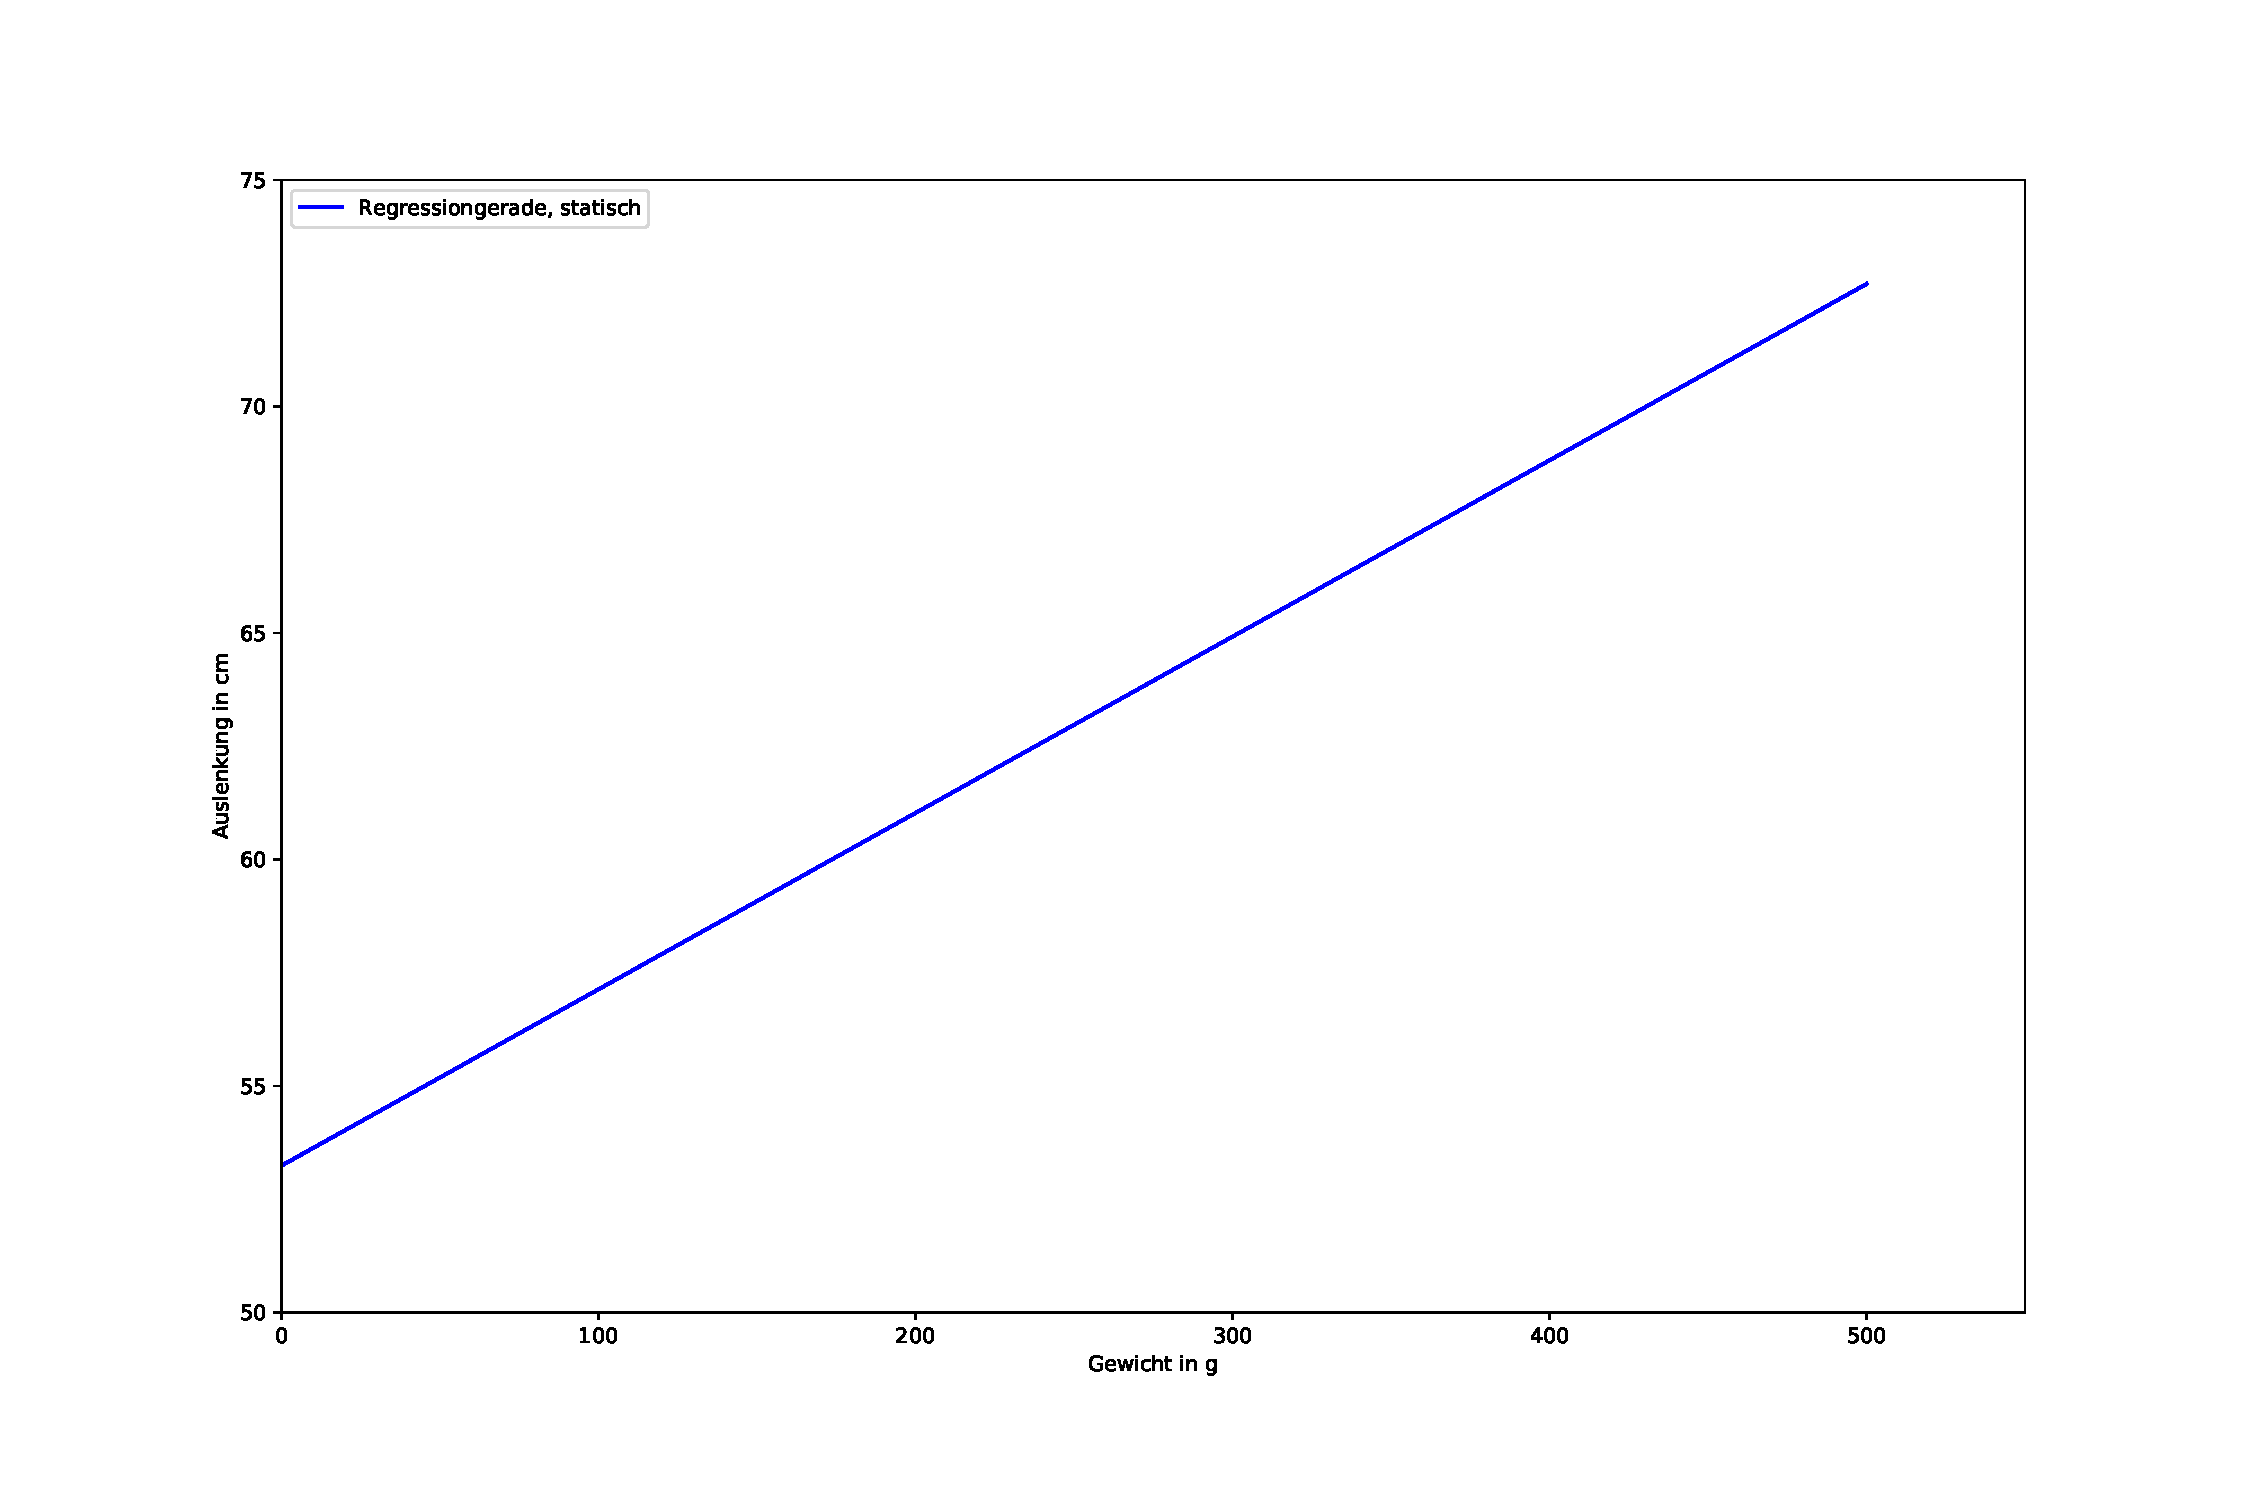
\includegraphics[scale = 0.4]{./Pendel/Protokoll/fig/Federkonstante_1.pdf}
        \caption{Regression der Schwingungsdauern der gekoppelten Oszillatoren,  Kopplungslänge 31cm}
        \label{fig:Schwingungsdauern-gekoppelte-Oszillatoren1}
    \end{center}
\end{figure}

\begin{figure}[h!]{}
    \begin{center}
        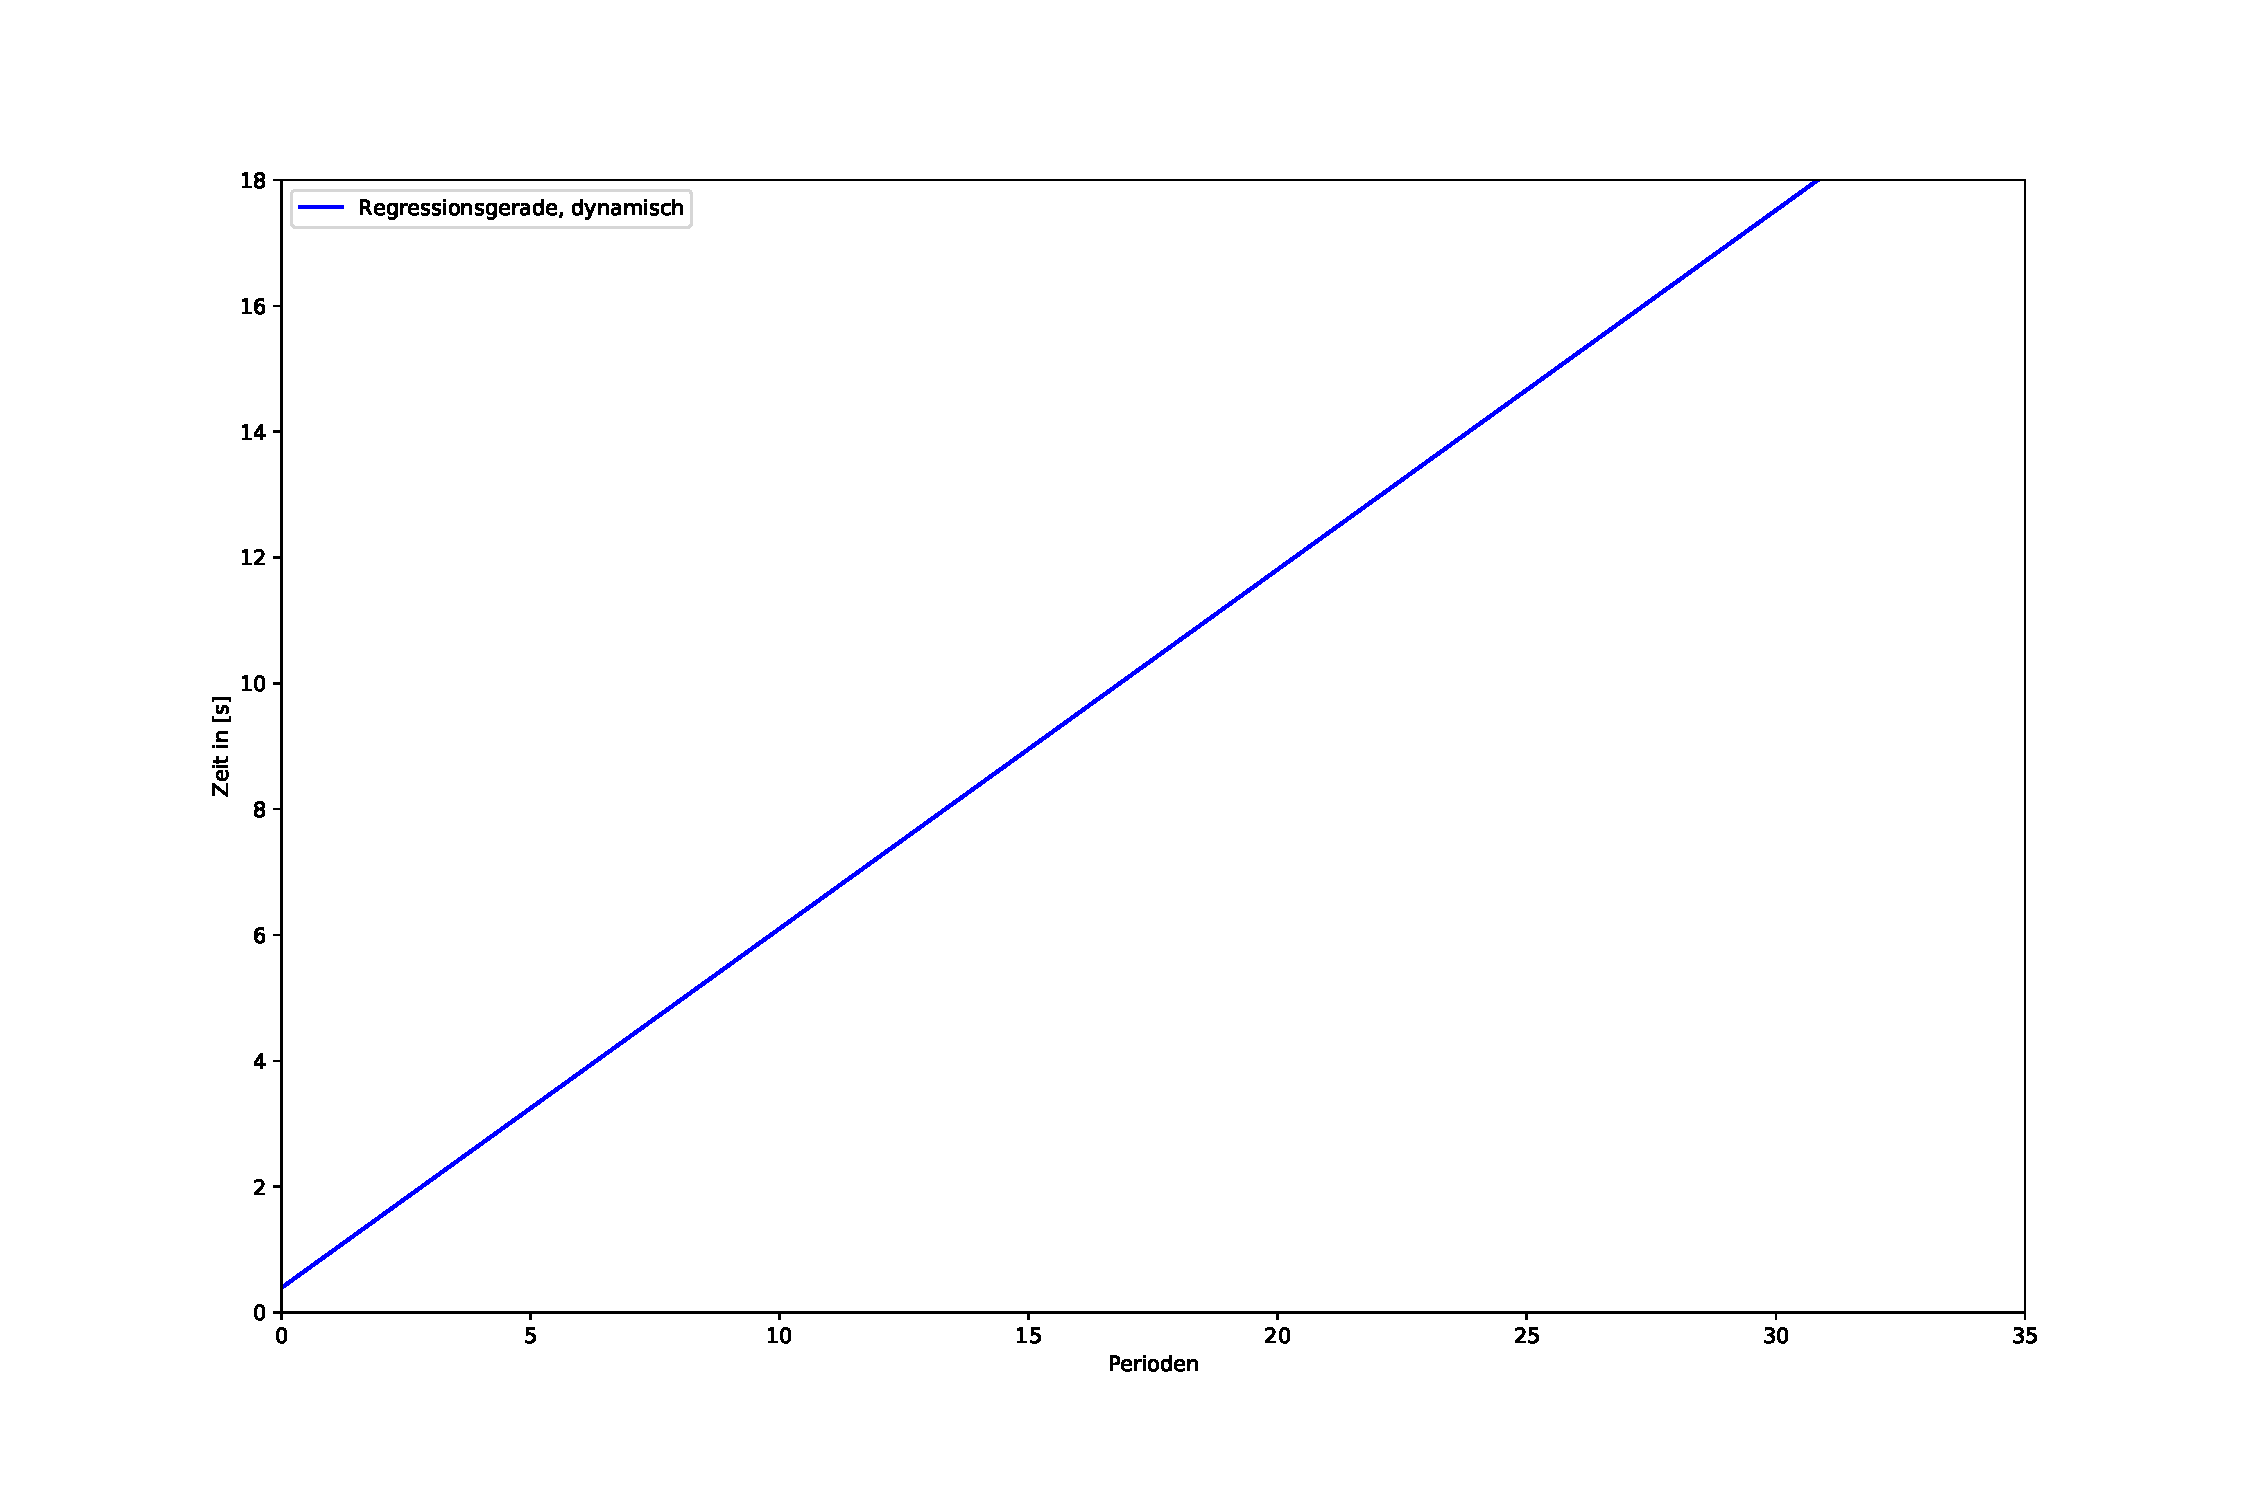
\includegraphics[scale=0.4]{./Pendel/Protokoll/fig/Federkonstante_2.pdf}
        \caption{Regression der Schwingungsdauern der gekoppelten Oszillatoren, Kopplungslänge 28cm}
        \label{fig:Schwingungsdauern-gekoppelte-Oszillatoren2}
    \end{center}
\end{figure}

Statisch ergibt sich mit eine Federkonstante von

\begin{equation}
    D = \frac{m \cdot g}{x} =\SI{17,21}{\frac{N}{m}} = 
\end{equation}

Dynamisch ergibt sich eine Federkonstante von

\begin{equation}
    D = 4 \cdot \pi^2 \frac{m}{T^2} = \SI{60,75}{\frac{N}{m}}
\end{equation}

Schwingungs- und Schwebungsdauer gekoppelter Oszillatoren

Nun werden noch die Schwingungs- und die Schwebungsdauer des gekoppelten Pendels aus blubba gemessen.
Dazu wird ein Pendel ausgelenkt, während das andere in Ruhe verbleibt.

\begin{table}[h]
    \begin{center}
        \caption{Schwingungs- und Schwebungsdauer}
        \begin{tabular}{cccc}
            \hline
            Periodenanzahl & Schwingungsdauer in $\SI{}{s}$ & Schwebungsdauer in $\SI{}{s}$ \\
            \hline
            $\SI{}{}$ & $\SI{}{}$ & $\SI{}{}$ \\
            $\SI{3}{}$ & $\SI{5,08 }{}$ & $\SI{44,19 }{}$ \\
            $\SI{5}{}$ & $\SI{8,59 }{}$ & $\SI{115,41}{}$ \\
            $\SI{7}{}$ & $\SI{11,70}{}$ & $\SI{144,49}{}$ \\
            $\SI{9}{}$ & $\SI{15,74}{}$ &  \\
            \hline
            \label{tab:Feder-dynamisch-Messwerte}
        \end{tabular}
    \end{center}
\end{table}

Zur Auswertung wurde erneut Regression verwendet, das Ergebnis für die Schwingungsdauer lautet $\SI{1.75(04)}{s}$, das für die Schwebungsdauer $\SI{24.34(389)}{s}$.
    
    %\chapter{Auswertung}
    %Ganz tolle Auswertung des Versuchs. \cite{Dem10} %\cleardoublepage

    % appendix for more or less interesting calculations
    %\Appendix
    %\chapter*{\appendixname} \addcontentsline{toc}{chapter}{\appendixname}
    % to make the appendix appear in ToC without number. \appendixname = 
    % Appendix or Anhang (depending on chosen language)
    %\section{Erster Abschnitt des Anhangs}
Dies ist der erste ganz tolle Abschnitt des Anhangs. %\cleardoublepage



    % Bibliography
    \TheBibliography
    % BIBTEX
    % use if you want citations to appear even if they are not referenced to: 
    % \nocite{*} or maybe \nocite{Kon64,And59} for specific entries
    %\nocite{*}
    \bibliographystyle{babalpha}
    \bibliography{lit.bib}

    % THEBIBLIOGRAPHY
    \begin{thebibliography}{000}
    %    \bibitem{ident}Entry into Bibliography.
    \bibitem{} Vorbereitungsmappe Pendel
    \end{thebibliography}
\end{document}
